% !TEX root = ../thesis-example.tex
%
\section{Virtual Z Sorting}

\todo[inline]{here a recap image of current steps: keying + delaying}

We have now a properly keyed video feed and synchronous motion between the VR 
actor and the 3D environment. To increase the immersion of that composition the 
next important step is to sort the scene on a tri-graph of planes.

\begin{figure}[htb]
	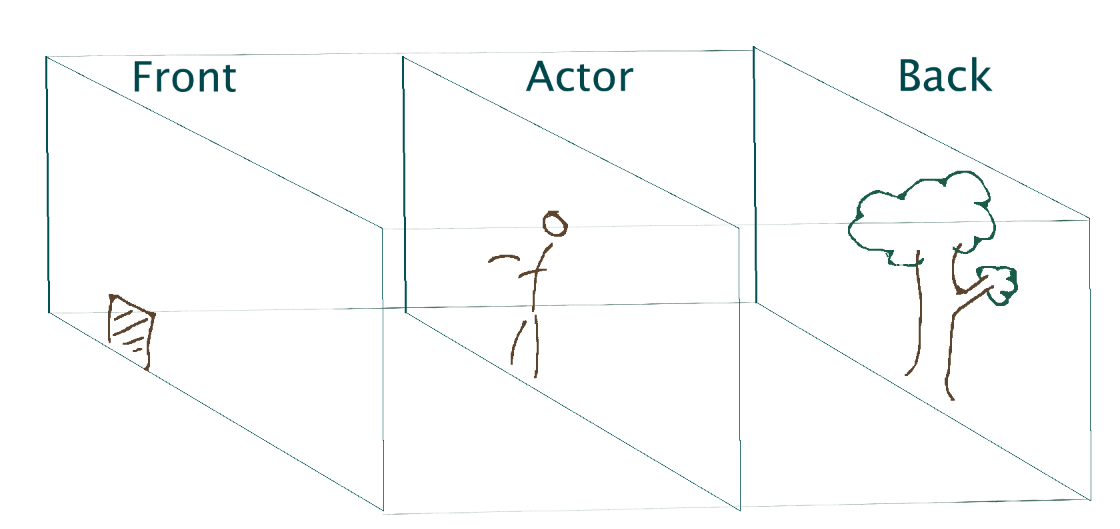
\includegraphics[width=\textwidth]{_raw_resources/composition/Composition-TriGraph.png}
	\caption{A sketch of the video composition with three layers of projection}
	\label{fig:zsort:sketch}
\end{figure}

There are multiple ways to achieve proper segmentation and composition of all 
three layers, depending on the rendering method. Deferred shading allows for 
better lightning simulation in engine but changes alpha- and depthmaps of a 
rendered scenery - this yields incorrect layer blending and results into an 
incorrectly displayed image. This software takes account for this and lets 
creators decide between two render modes:

\begin{my_list}
	\item Replace Masking: A front plane is displayed, after it follow the 
	chroma-keyed video and then the background. This is the most accurate image 
	generation.
	\item Alpha Masking: A front alpha mask of the geometry is displayed, then 
	the actor is mixed with a full render image of the background. The 
	resulting image has inconsistencies with alpha-blending but this method 
	works with all rendering setups.
\end{my_list}

The decision is between accuracy and presentation. Many post processing effects 
or deferred shading are not able - or simply do not respect - the alpha matte, 
which is usually no issue, since these steps are taken after rendering is 
complete, thus causing no unwanted side-effects. Other post effects need 
certain projection requirements and / or get disregarded through culling, like 
in Figure \ref{fig:zsort:comparison:front} where the volumetric lightning is 
culled out of the virtual projection and therefore gets completely ignored, 
resulting in a black front geometry.

\begin{figure}[htbp]
	\caption{A comparison of different composition methods in engine}
	\label{fig:zsort:comparison}
	\begin{subfigure}[t]{.45\textwidth}
		\centering
		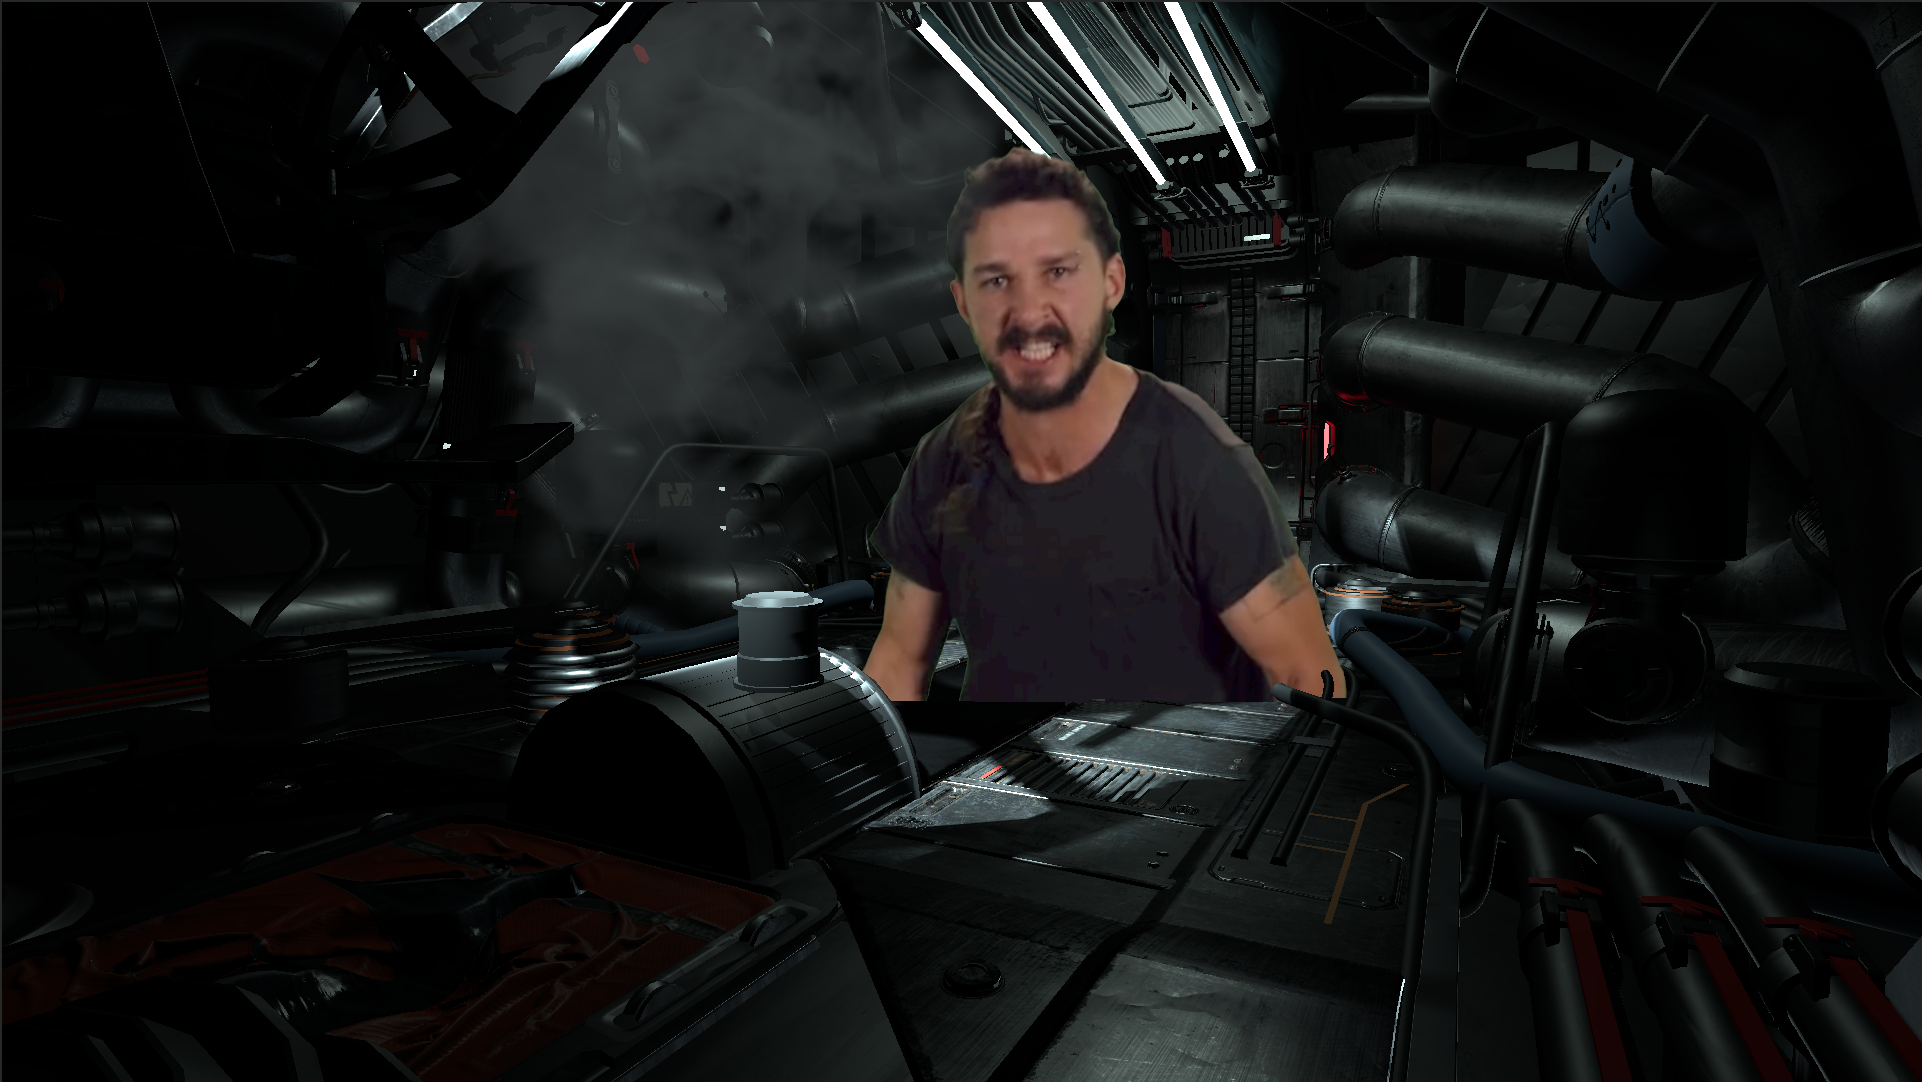
\includegraphics[width=\textwidth]{_raw_resources/composition/Composition-Perfect-Realigned.png}
		\caption{The proposed composition, simulated, with an arbitrary depth 
		of the video feed}
	\end{subfigure}
	\begin{subfigure}[t]{.45\textwidth}
		\centering
		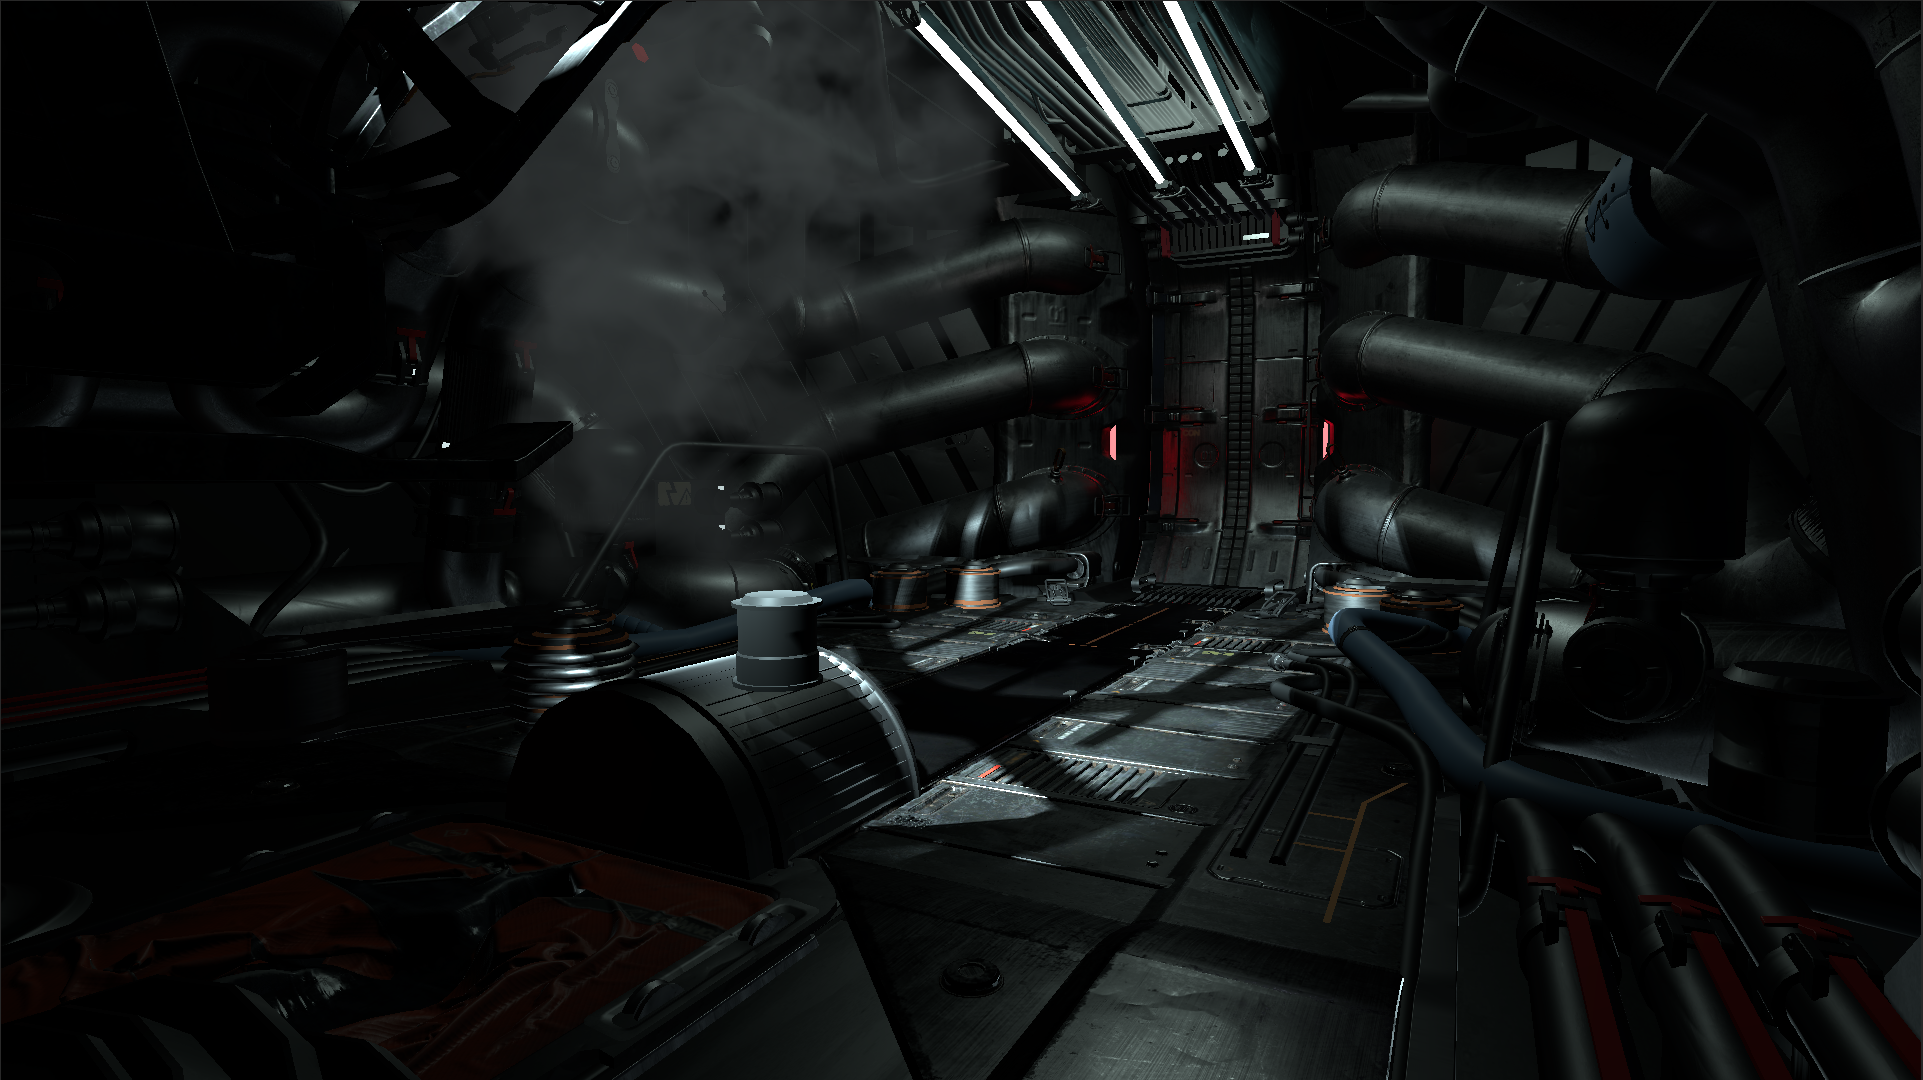
\includegraphics[width=\textwidth]{_raw_resources/composition/Composition-Full-Render.png}
		\caption{The full length rendering}
	\end{subfigure}
	\newline
	\begin{subfigure}[t]{.45\textwidth}
		\centering
		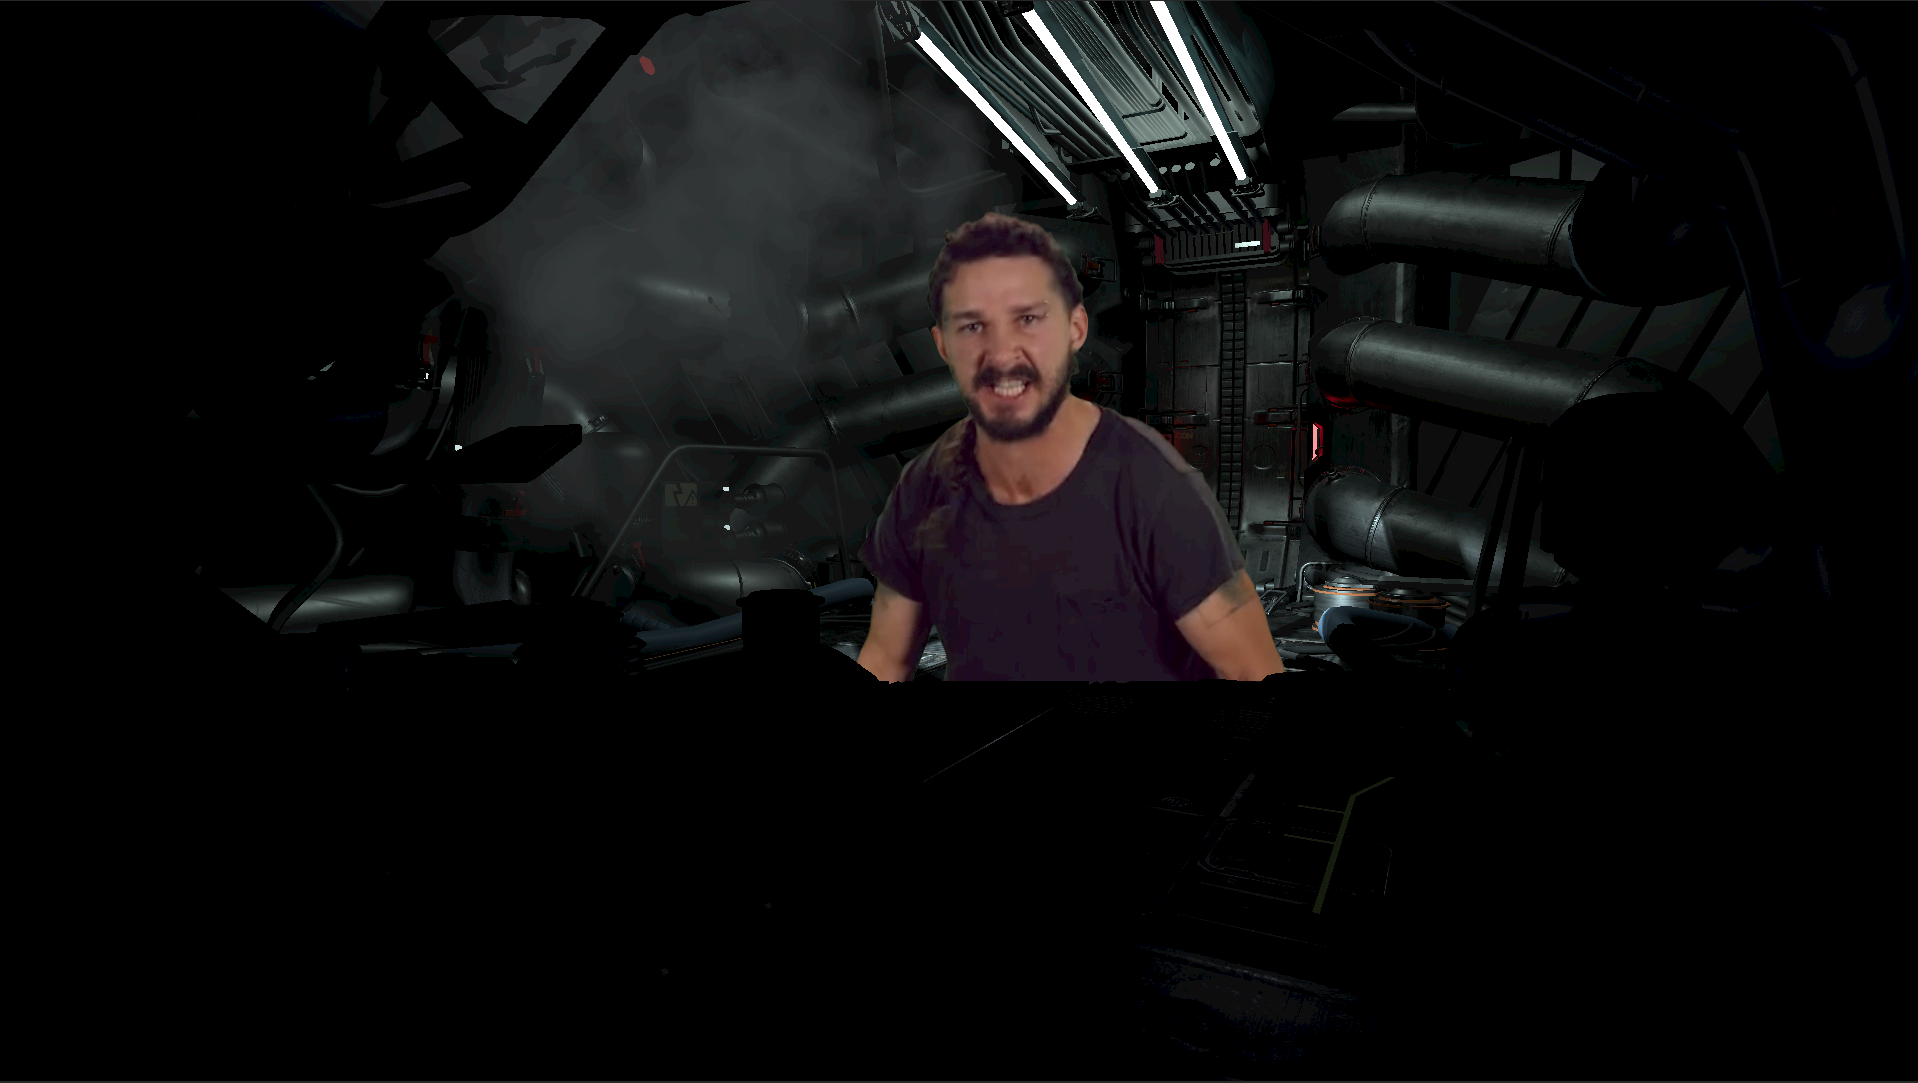
\includegraphics[width=\textwidth]{_raw_resources/composition/Composition-Front-Replace_orso.png}
		\caption{A composition by rendering a front, followed by the video and 
		then the background}
	\end{subfigure}
	\begin{subfigure}[t]{.45\textwidth}
		\centering
		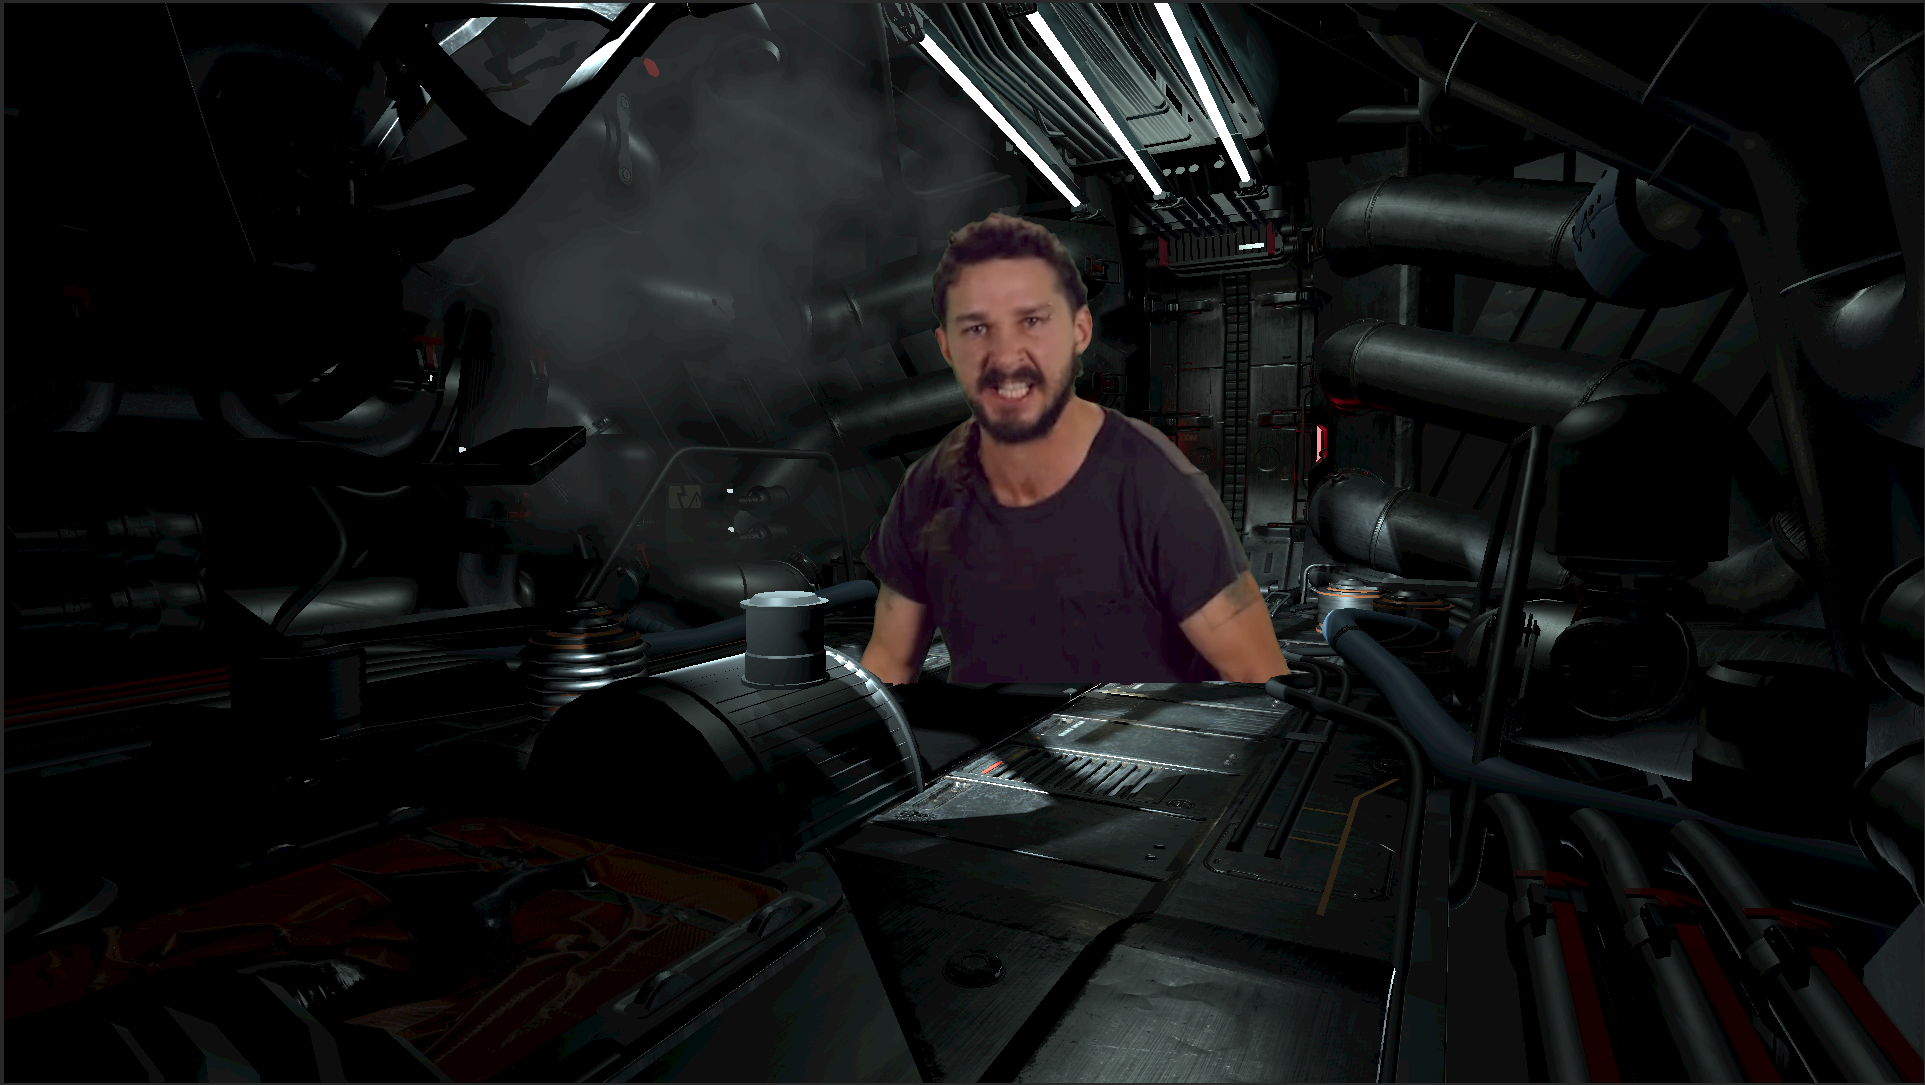
\includegraphics[width=\textwidth]{_raw_resources/composition/Composition-Front-Mask.png}
		\caption{A composition with the front geometry as mask, and then a 
		mixing of the video and a full length render}
	\end{subfigure}
	\newline
	\begin{subfigure}[t]{.45\textwidth}
		\centering
		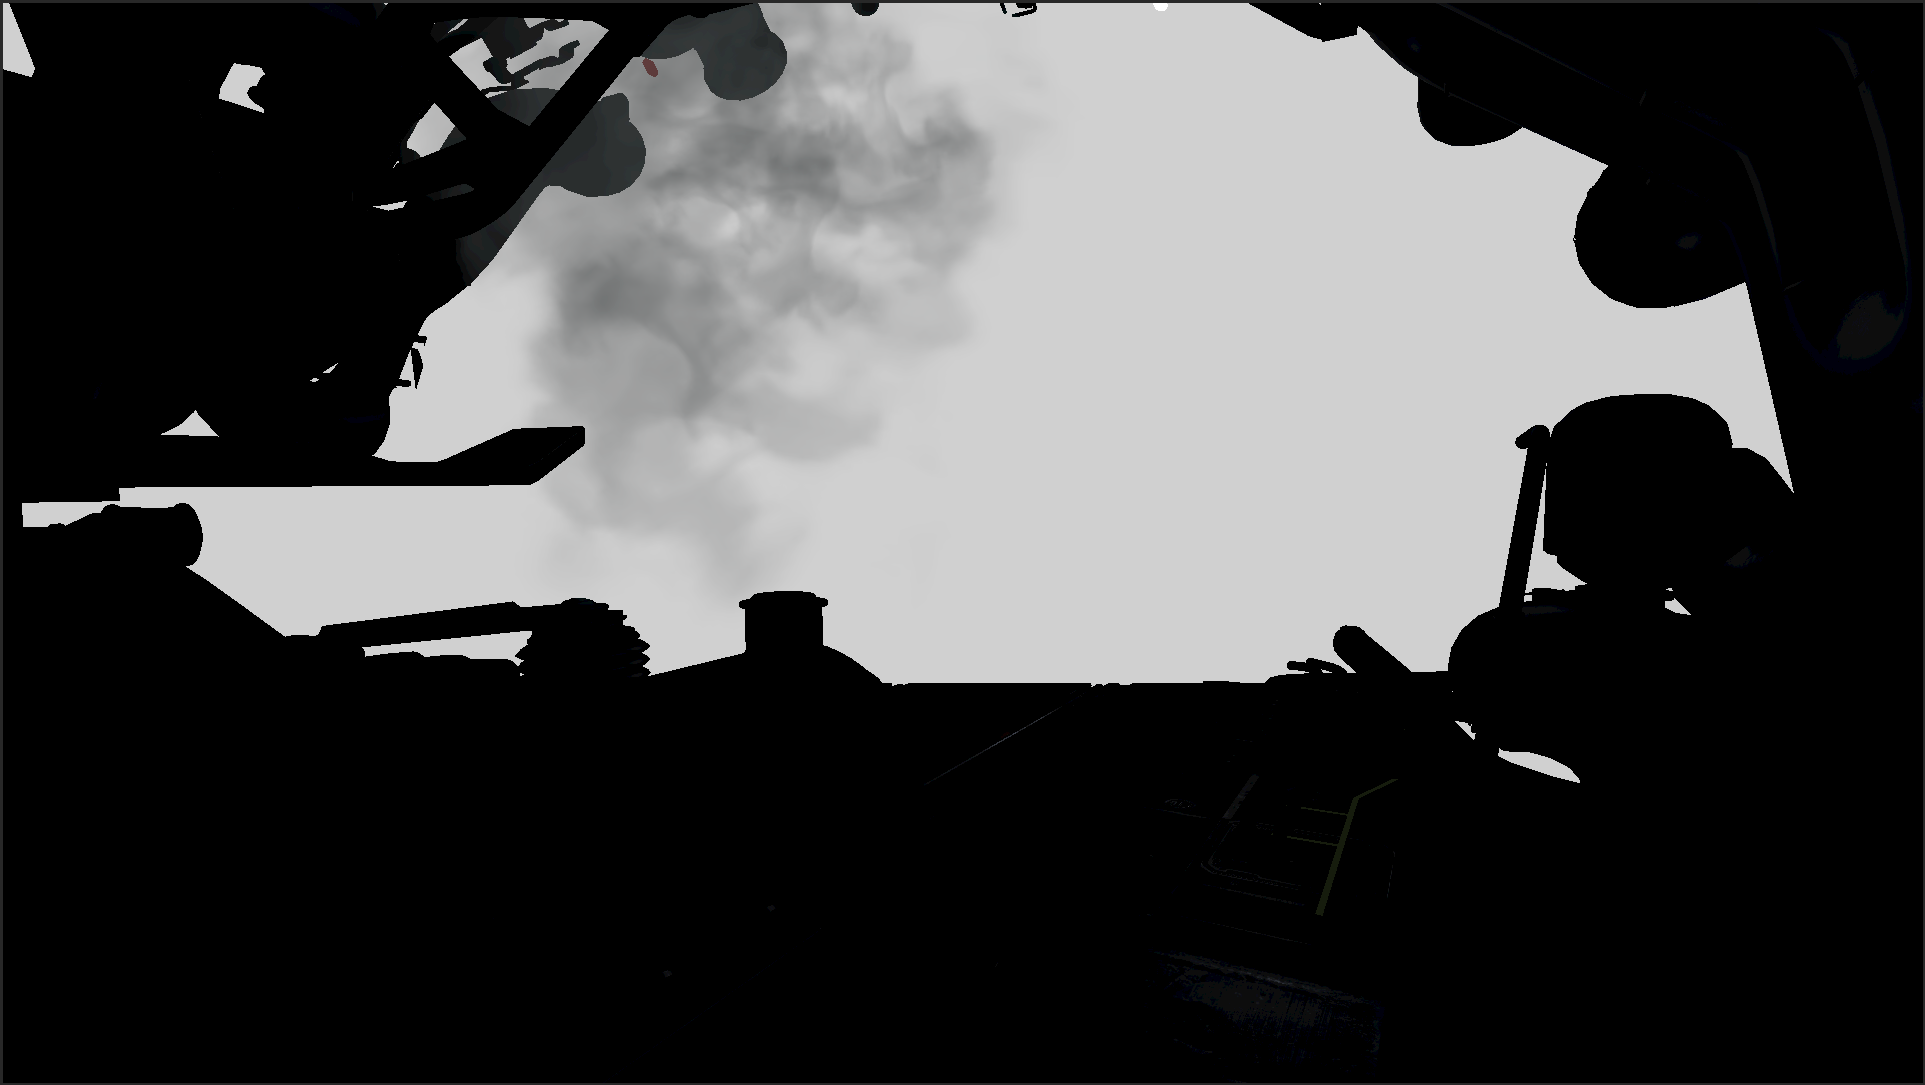
\includegraphics[width=\textwidth]{_raw_resources/composition/Composition-Front.png}
		\caption{The virtual projection of the front camera - volumetric 
		lightning does not work due to the short projection length}
		\label{fig:zsort:comparison:front}
	\end{subfigure}
	\begin{subfigure}[t]{.45\textwidth}
		\centering
		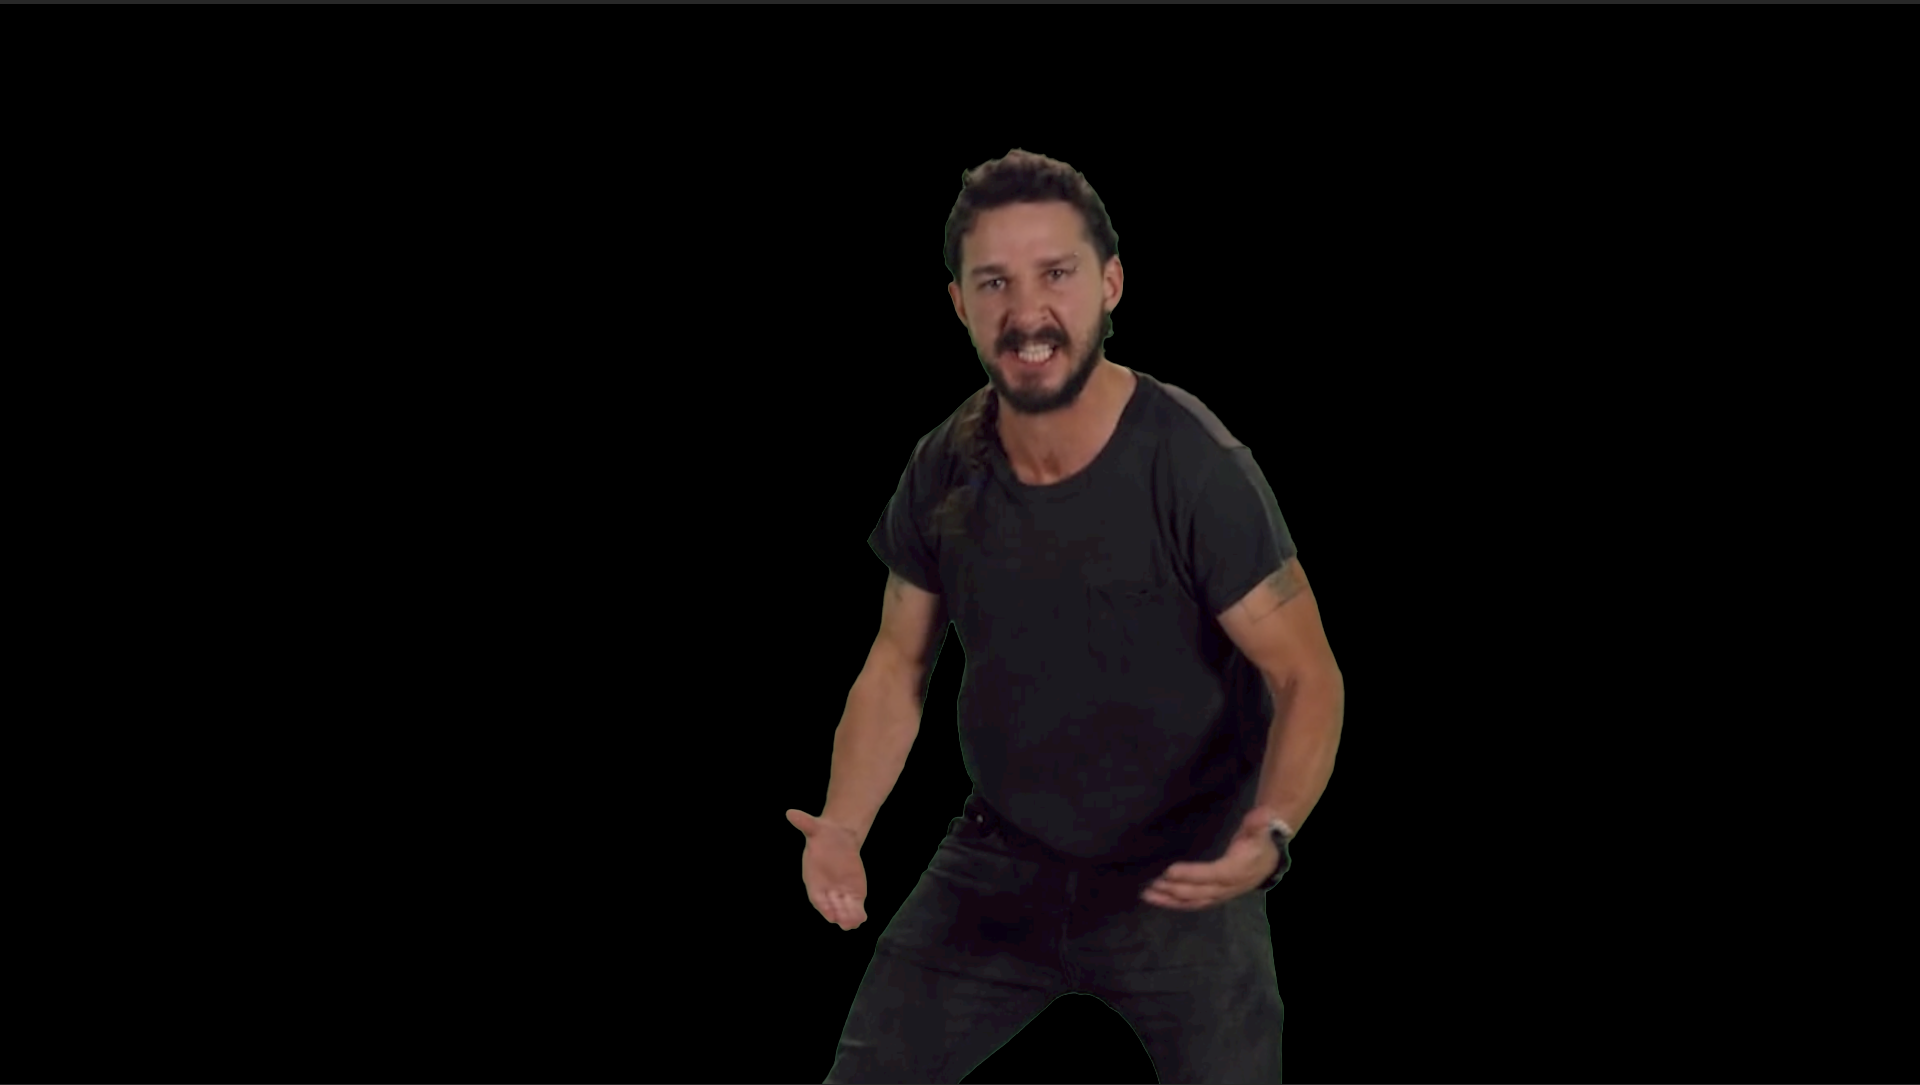
\includegraphics[width=\textwidth]{_raw_resources/composition/Composition-Chroma-Result.png}
		\caption{The chroma keying result}
	\end{subfigure}
\end{figure}

Mixing these three layers are similarly easy, using a previous equation 
\eqref{eq:chroma:assumption:alpha:weak} and 
\eqref{eq:chroma:assumption:alpha:cont}. Assuming an ARGB front render image 
$F$, a RGB video feed  $V$ and the RGB background $B$, 
we can mix all three layers effortlessly:

Replace Masking:

\eq{eq:zsort:replmask:1}{
	\alpha_T = \alpha_V * (1 - \alpha_F)
}


\eq{eq:zsort:replmask:2}{
	I(x, y) = (1 - \alpha_T) * F(x, y) + \alpha_T * V(x, y)
}

\eq{eq:zsort:replmask:3}{
	\alpha_S = \alpha_B * (1 - \alpha_{I(x, y)})
}


\eq{eq:zsort:replmask:2}{
	J(x, y) = (1 - \alpha_S) * I(x, y) + \alpha_S * B(x, y)
}

Alpha Masking is very similar with transforming the alpha-mask of the webcam 
footage after chroma-keying it. It is masking the video further, after the 
video matte is pulled already:

\eq{eq:zsort:alphamask:1}{
	\alpha_{V_T} = 
	\begin{cases}
		1 - \alpha_F  & \quad \text{if } \alpha_V > 0 \\
		\alpha_V      & \quad \text{otherwise}
	\end{cases}	
}

\todo[inline]{This is a bit incorrect as what is currently used in the shader.}

\eq{eq:zsort:alphamask:2}{
	\alpha_T =  \alpha_B * (1 - \alpha_{V_T})
}

\eq{eq:zsort:replmask:2}{
	I(x, y) = (1 - \alpha_T) * V(x, y) + \alpha_T * B(x, y)
}

\todo[inline]{remindme: there is the depth-offset missing currently.}

Now we have a well mixed image composition where the actor is placed in between 
two projections and thus can have an interactive fore- and background. The 
initial assumption is, that the actors depth is flattened, based on the 
distance between a real world camera and the Vive Head Mounted Display.
